\documentclass{article}
\usepackage{graphicx}
\usepackage[utf8]{inputenc}
\usepackage{amsmath, amssymb, latexsym}

\usepackage{pgfplots}
\usepackage{algorithm}
\usepackage[noend]{algpseudocode}
\usepackage{tikz}
\usepackage{nicefrac}
\usepackage{placeins}
\pgfplotsset{every axis legend/.append style={
at={(0,0)},
anchor=north east}}
\usetikzlibrary{shapes,positioning,intersections,quotes}
\usetikzlibrary{arrows.meta,
                bending,
                intersections,
                quotes,
                shapes.geometric}
                
\definecolor{darkgreen}{rgb}{0.0, 0.6, 0.0}
\definecolor{darkred}{rgb}{0.7, 0.0, 0.0}
\makeatletter
\def\BState{\State\hskip-\ALG@thistlm}
\makeatother
\title{Week 15}
\begin{document}
\pagenumbering{gobble}
\maketitle
\newpage
\pagenumbering{arabic}

\section*{Anomaly detection}

\begin{itemize}
  \item We can assess whether data points are anomalous by using the dataset as a baseline.
  \item if $p(x_{test}) < \epsilon \quad$, then flag this as an anomaly
  \item if $p(x_{test}) \geq \epsilon \quad$, then this is OK
  \item $\epsilon$ is a threshold probability number that we determine based on how certain we need/want to be.
\end{itemize}

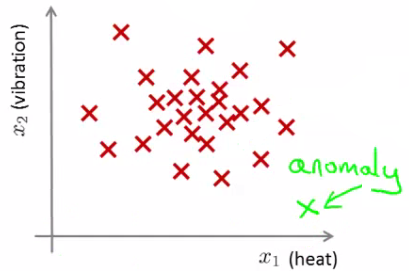
\includegraphics[width=0.5\textwidth]{resources/anomaly}

\section*{Applications}
\begin{itemize}
  \item Fraud detection

        \begin{itemize}
          \item Users have activities connected with them, such as the amount of time spent online, the location of login, and the frequency with which they spend money.
          \item Using this information, we can create a model of what regular users do.
          \item What is the probability of "normal" behavior?
          \item Send atypical users' data through the model to identify them. Make a note of everything that appears unusual. Block cards/transactions automatically.
        \end{itemize}

  \item Manufacturing

        \begin{itemize}
          \item Aircraft engine example.

        \end{itemize}

  \item Monitoring computers in data center

        \begin{itemize}
          \item If you have many machines in a cluster (x1 = memory use, x2 = number of disk accesses/sec, x3 = CPU load).
          \item When you notice an anomalous machine, it is likely that it is soon to fail.
          \item Consider replacing parts of it.
        \end{itemize}
\end{itemize}

\section*{The Gaussian distribution}

\begin{itemize}
  \item $\mu$ is mean.
  \item $\sigma^2$ is variance and $\sigma$ is a standard deviation.
  \item probability of x, parameterized by the mean and variance:
\end{itemize}

$$p(x; \mu; \sigma^2) = \frac{1}{\sqrt{2\pi\sigma}}exp(-\frac{(x-\mu)^2}{2\sigma^2})$$

~\\

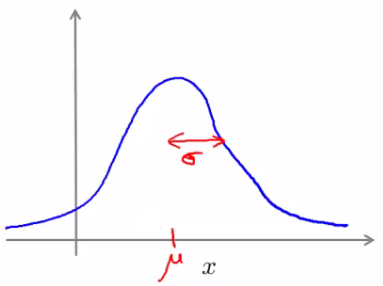
\includegraphics[width=0.5\textwidth]{resources/gaussian}

\begin{itemize}
  \item Assume we have a data collection of m examples.
  \item Given that each example is a real number, we plot the data on the x axis.
  \item Given the dataset can you estimate the distribution?
\end{itemize}

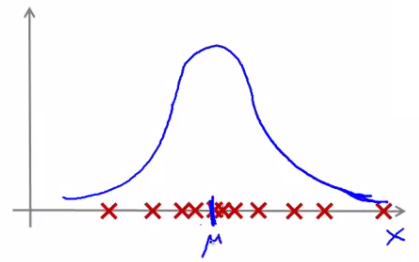
\includegraphics[width=0.6\textwidth]{resources/data_fit}

Seems like a good fit - data suggests a higher likelihood of being in the center and a lower likelihood of being further out.

\newpage
\section*{Anomaly detection}

\FloatBarrier
\begin{algorithm}
\caption{Anomaly detection}\label{euclid}
\begin{algorithmic}[1]
\State Choose features $x_i$ that you think might be indicative of anomalous examples.
\State Fit parameters $\mu_1, ..., \mu_n, \sigma_1^2, ..., \sigma^n$

$$\mu_j = \frac{1}{m} \sum_{i=1}^mx_j^{(i)}$$
$$\sigma_j^2 = \frac{1}{m} \sum_{i=1}^m(x_j^{(i)}-\mu_j)^2$$

\State Given new example x, compute p(x):

$$p(x)= \prod_{j=1}^n \frac{1}{\sqrt{2\pi\sigma_j}}exp(-\frac{(x_j-\mu_j)^2}{2\sigma_j^2})$$

\end{algorithmic}
\end{algorithm}
\FloatBarrier

\section*{Developing and evaluating and anomaly detection system}

\begin{itemize}
  \item You have some labeled data.

        \begin{itemize}
          \item $y=0$ for engines which were non-anomalous.
          \item $y=1$ for engines which were anomalous.
        \end{itemize}

  \item Training set is the collection of normal examples.
  \item Next define:

        \begin{itemize}
          \item Cross validation set.
          \item Test set.
          \item For both assume you can include a few examples which have anomalous examples.
        \end{itemize}

  \item In our example we have:

        \begin{itemize}
          \item 10000 good engines.
          \item 50 flawed engines.
        \end{itemize}
        
  \item Split into:

        \begin{itemize}
          \item Training set: 6000 good engines (y = 0).
          \item CV set: 2000 good engines, 10 anomalous.
          \item Test set: 2000 good engines, 10 anomalous.
        \end{itemize}
        
\end{itemize}


~\\
What's a good metric to use for evaluation?

\begin{itemize}
  \item Compute fraction of true positives/false positive/false negative/true negative.
  \item Compute precision/recall.
  \item Compute F1-score.
\end{itemize}

\section*{Multivariate Gaussian distribution}
It is a somewhat different approach that can occasionally discover anomalies that normal Gaussian distribution anomaly detection fails to detect.

\begin{itemize}
  \item Assume you can fit a Gaussian distribution to CPU load and memory use.
  \item Assume we have an example in the test set that appears to be an anomaly (e.g. x1 = 0.4, x2 = 1.5).
  \item Here memory use is high and CPU load is low (if we plot x1 vs. x2 our green example looks miles away from the others).
  \item The problem is that if we look at each characteristic individually, they may fall inside acceptable bounds - the difficulty is that we know we shouldn't obtain those types of numbers together, but they're both okay individually.
\end{itemize}

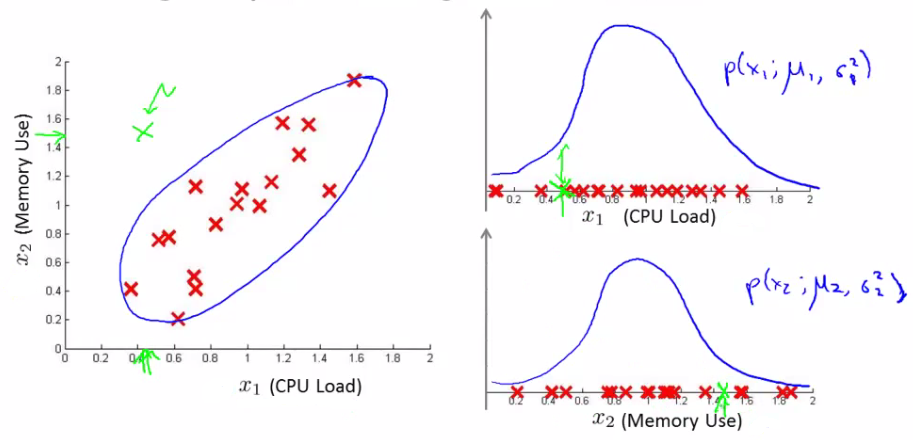
\includegraphics[width=\textwidth]{resources/mult_gauss}

~\\
What are the parameters for this new model?
\begin{itemize}
  \item $\mu$ which is an n dimensional vector (where n is number of features)
  \item $\Sigma$ which is an [n x n] matrix - the covariance matrix
\end{itemize}

$$p(x; \mu; \Sigma) = \frac{1}{(2\pi)^{n/2}|\Sigma|^{1/2}}exp(-\frac{1}{2}(x-\mu)^T \Sigma^{-1}(x-\mu))$$

~\\\\
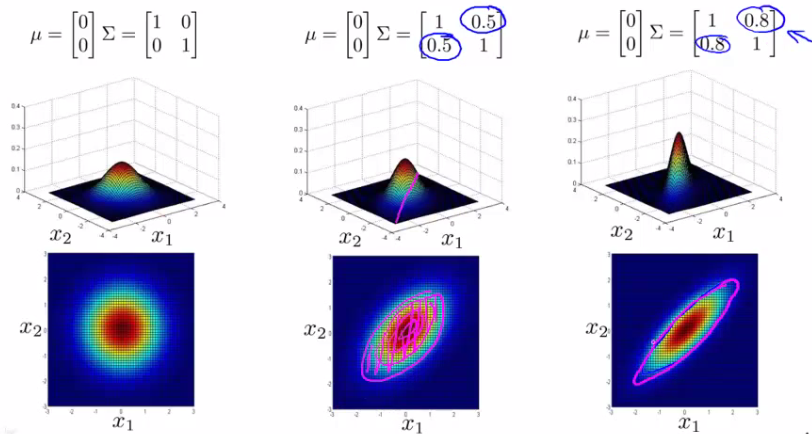
\includegraphics[width=\textwidth]{resources/cov_matrix_sigma}

~\\
Very tall thin distribution, shows a strong positive correlation.

\subsection*{Gaussian model - summary}

\begin{itemize}
  \item Probably used more often.
  \item There is a need to manually create features to capture anomalies where x1 and x2 take unusual combinations of values.
  \item So need to make extra features and might not be obvious what they should be.
  \item Much cheaper computationally.
  \item Scales much better to very large feature vectors.
  \item Works well even with a small training set e.g. 50, 100.
\end{itemize}


\subsection*{Multivariate gaussian model - summary}

\begin{itemize}
  \item Used less frequently.
  \item Can capture feature correlation.
  \item So no need to create extra values.
  \item Less computationally efficient.
  \item Needs for m > n  i.e. number of examples must be greater than number of features.  
\end{itemize}


\end{document}